\documentclass{article}
\usepackage{graphicx}
\graphicspath{ {imgs/} }
\usepackage[utf8]{inputenc}
\usepackage[brazil]{babel}
\usepackage[a4paper, left=20mm, right=20mm, top=20mm, bottom=20mm]{geometry}
\usepackage[colorlinks, urlcolor=blue, citecolor=red]{hyperref}

\title{\textbf{INE5430 - Inteligência Artificial \\
        \large Trabalho T5 - Redes Neurais}}
\author{
    Caique Rodrigues Marques \\
    {\texttt{c.r.marques@grad.ufsc.br}}
    \and
    Fernando Jorge Mota \\
    {\texttt{contato@fjorgemota.com}}
    \vspace{-5mm}
}
\date{}
\begin{document}
    \maketitle
    
    \section*{Introdução}
        A tarefa de reconhecimento de dígitos manuscritos é uma tarefa simples
        para o cérebro humano e para alguns animais. Infelizmente, para um
        computador, essa tarefa não é algo tão simples de ser programada, pois
        um digito pode ser representado de maneiras que, embora semelhantes aos
        olhos humanos, são de fato diferentes do ponto de vista determinístico,
        mesmo que sejam apenas alguns poucos pixeis de diferença.
        
        Além disso, outro problema comum que também acontece relacionado à
        tarefa de reconhecimento de dígitos é identificar um em específico a
        partir de uma imagem, sendo que o dígito representado na imagem pode se
        parecer bastante com um outro distinto - isto também acontece ao olho
        humano - exemplos são números como 3 e 9 ou 9 e 8, que dependendo de
        sua representação podem ser visualmente parecidos.
        
        Dado todas essas informações, fica claro que o reconhecimento de
        dígitos manuscritos não é, de fato, algo que pode ser desenvolvido de
        maneira computacionalmente simples. É complicado, na prática, programar
        um algoritmo direto que seja capaz de analisar a entrada de uma imagem
        e retornar que digito é, acompanhado de sua probabilidade definida,
        portanto, para este tipo de tarefa, normalmente é escolhido o uso de
        redes neurais.
        
        Com o uso de redes neurais, é possível dar ao programa um "conjunto de
        treinamento" composto por imagens (representada através de uma lista de
        pixeis da imagem) e seus respectivos dígitos e, a partir desse
        conjunto, fazer o programa inferir que digito corresponde a uma
        determinada imagem, identificando os padrões correspondentes.
        
        A partir do conjunto de treinamento, é aplicado as imagens de um
        conjunto de teste e é verificado a taxa de acerto comparando os dígitos
        que eles realmente representavam com o que o programa detectou.
    
    \section*{O sistema e a análise}
        O programa \texttt{mnist\_analyser.py} \footnote{O arquivo
        \texttt{requirements.txt} define as dependências necessárias para a
        execução do programa.}, que realiza a avaliação dos dígitos
        manuscritos, foi escrito com a linguagem de programação Python,
        juntamente com a biblioteca
        \href{http://scikit-learn.org/stable/index.html}{\texttt{scikit-learn}}
        que fornece as ferramentas para a manipulação e administração das redes
        neurais. Os dados que o programa analisa estão no formato CSV, com 401
        linhas e 5000 colunas, sendo que cada coluna representa um padrão de
        pixeis numa matriz de 20x20 e a última linha corresponde ao dígito em
        questão dos pixeis especificados nas colunas.
        
        A análise é feita, primeiramente, separando o conjunto dos dados em
        conjunto de treinamento e em um conjunto de testes, sendo que $75\%$
        dos dados são usados para treinamento e os $25\%$ restante são usados
        para teste. Esse conjunto é selecionado de maneira uniforme por digito,
        ou seja, $75\%$ das amostras relacionadas a cada digito são processadas
        separadamente, de forma a evitar que a distribuição dos conjuntos de
        captura e de teste varie conforme os dígitos.
        
        Além de ser feita de maneira uniforme, a amostragem é feita de maneira
        aleatória. Ou seja, dado um \textit{seed} (de forma que a
        reprodutibilidade dos testes é mantida), o programa coleta as amostras
        usando um gerador de números pseudoaleatórios para que diferentes itens
        do conjunto sejam treinados e não apenas um intervalo continuo entre um
        número e outro de amostras, por exemplo, garantindo assim maior
        diversidade nos testes.
    
    \section*{Métodos utilizados}
        Após a separação dos conjuntos de testes e treinamentos, a avaliação de
        tais dados é feita usando um classificador \textit{Multi-Layer
        Perceptron}, onde a rede neural possui camadas escondidas compostas por
        um definido número de neurônios. O classificador MLP tem a forma de um
        grafo acíclico direcionado, ou seja, não há ciclos (informações de uma
        camada a frente não são repassados para trás) e seguem um caminho
        (percorre as camadas, sem saltos). No programa, o classificador MLP é
        utilizado com a classe \texttt{MLPClassifier}, provinda pela biblioteca
        \texttt{scikit-learn}.
        
        Dos testes realizados, o melhor resultado obtido até então envolve o
        uso de duas camadas escondidas, com 100 neurônios em cada uma; taxa de
        aprendizado de $0.035$, usando o método de taxa de aprendizado
        adaptativa caso a taxa de perdas tenha variação menos do que $0.0001$;
        função sigmoidal ou função logística como função de ativação; para o
        método para a otimização dos pesos (\textit{solver}) foi usado o
        algoritmo de Broyden–Fletcher–Goldfarb–Shanno (BFGS) e foi estabelecido
        no máximo 200 iterações para a rede neural. 
        
        \subsection*{Testes}    
            Até chegar nesse resultado, foram realizados diferentes tipos de
            teste, com diferentes parâmetros da rede. Foram testados variações
            da taxa de aprendizado, entre $0.1$ e $0.05$, testando com
            diferentes algoritmos como o gradiente descendente estocástico para
            a otimização de pesos (ou seja, como \textit{solver}) e a função de
            ativação de unidade linear retificada. Entretanto, tais testes não
            se provaram tão eficientes quanto os parâmetros escolhidos,
            deixando a desejar tanto em questão de velocidade quanto em questão
            de performance. Com estas métricas, a rede demorava mais para
            convergir, chegando a rodar todas as 200 iterações e tendo como
            taxa de acertos entre $91\%$ e $92\%$.
        
        \subsection*{Avaliação}
            Para análise da performance da rede neural foram estabelecidos duas
            formas de avaliação:
            \begin{itemize}
                \item Matriz de confusão, mostrando o índice de acertos e erros
                    por cada número e quantos neurônios erraram ou acertaram.
                    Disto é possível tirar o cálculo da taxa de acertos (ou
                    análise dos verdadeiros positivos, definido como $TPR$),
                    mostrando o quanto, em porcentagem, a rede acertou de todas
                    as imagens apresentadas. O cálculo da taxa de erros também
                    é usado, sendo o inverso da taxa de acerto ($1 - TPR$);
                \item Uma visualização de imagens de treino e de teste e qual
                    foi a predição da respectiva imagem.
            \end{itemize}
            
            A seguir, um exemplo da saída do programa, com os parâmetros da
            rede neural especificados nesta seção. A taxa de acerto obtida foi
            de $92.64\%$, com 71 iterações, e a matriz de confusão pode ser
            vista na figura abaixo à esquerda, assim como um exemplo, à
            direita, do que a rede treinou e testou e qual a predição
            estabelecida.

            Pelos nossos testes, a saída do programa tem como taxa de acerto
            entre $92\%$ e $94\%$ e o número de iterações chega a ser menos de
            oitenta.

        \begin{figure}[!h]
            \centering
            \begin{minipage}[b]{0.5\textwidth}
                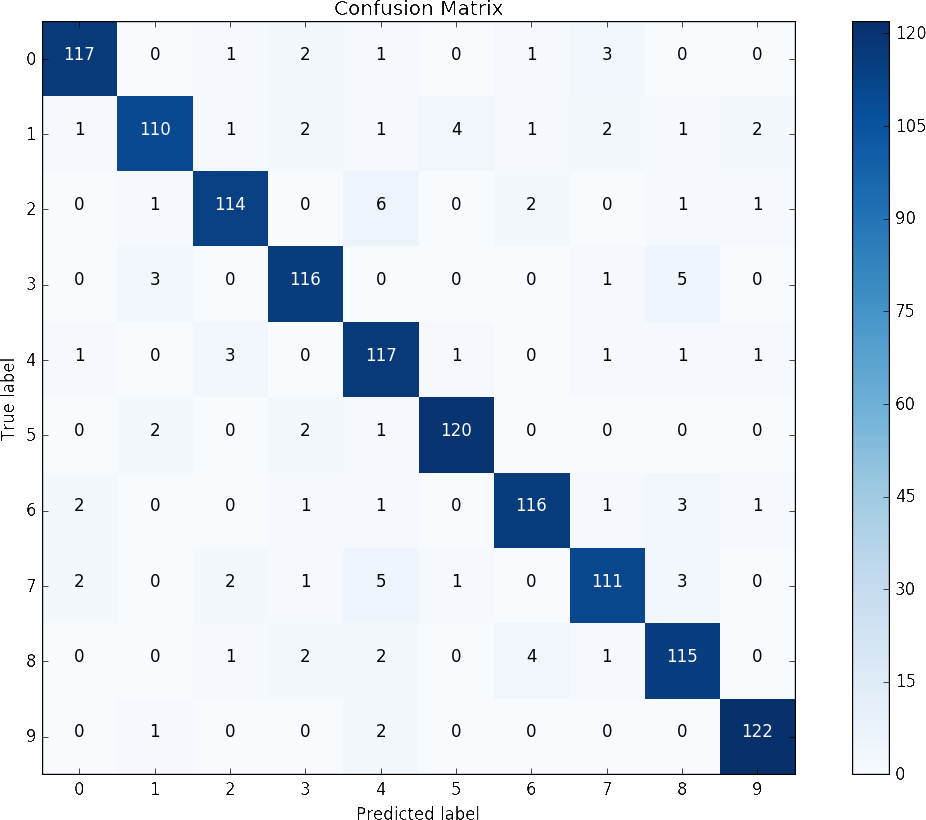
\includegraphics[width=\textwidth]{confusion_matrix.png}
                \caption{Matriz de confusão da avaliação dos dígitos
                manuscritos da base de dados MNIST}
            \end{minipage}
            \hfill
            \begin{minipage}[b]{0.4\textwidth}
                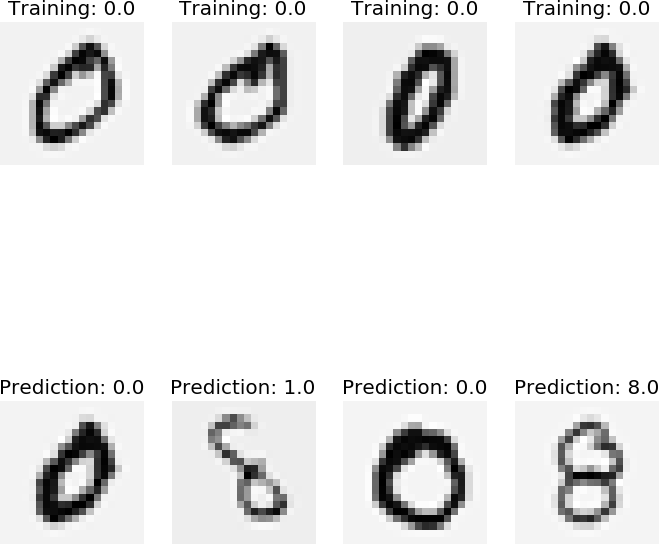
\includegraphics[width=\textwidth]{digits.png}
                \caption{Acima estão amostras dos dados de treinamento com os
                respectivos valores e abaixo estão amostras dos dados de teste
                com os valores preditos pela rede neural}
            \end{minipage}
        \end{figure}

\end{document}
